\documentclass[10pt]{article}
\usepackage[utf8]{inputenc}
\usepackage[T1]{fontenc}
\usepackage{amsmath}
\usepackage{amsfonts}
\usepackage{amssymb}
\usepackage[version=4]{mhchem}
\usepackage{stmaryrd}
\usepackage{graphicx}
\usepackage[export]{adjustbox}
\graphicspath{ {./images/} }
\usepackage{caption}

\begin{document}

\section*{Data Analysis 2: 'Isolated black hole'}
In 2022, two independent groups reported the discovery of an isolated black hole based on observations of the gravitational microlensing event OGLE-2011-BLG-0462. In this problem, we will analyze data from the Hubble Space Telescope to reproduce their findings.

Gravitational microlensing occurs when the light of a distant star (the 'source') is bent and magnified by the gravitational field of an intervening object (the 'lens'). The characteristic angular scale of gravitational microlensing events, called the angular Einstein radius $\theta_{\mathrm{E}}$, depends on the mass $M$ and distance $D_{\ell}$ from the Earth to the lens:

$$
\theta_{\mathrm{E}}=\sqrt{\frac{4 G M}{c^{2}} \frac{D_{s}-D_{\ell}}{D_{s} D_{\ell}}},
$$

where $D_{s}$ is the distance to the source star. For typical microlensing events observed in the Milky Way, the source stars are in the Galactic bulge, near the Galactic center, so $D_{s} \approx 8 \mathrm{kpc}$.\\
(a) Calculate the angular Einstein radius in milliarcseconds (mas) for an example lens of $1 M_{\odot}$ located at a distance of 1 kpc .\\
(2 points)\\
Suppose that at time $t$ the lens and the source are separated by an angle $\theta \equiv u(t) \theta_{\mathrm{E}}$ on the sky. Two images of the source are created on a line through the positions of the source and the lens, at angular distances $\theta_{+}$and $\theta_{-}$from the lens given by:

$$
\theta_{ \pm}=\frac{1}{2}\left(u \pm \sqrt{u^{2}+4}\right) \theta_{\mathrm{E}} .
$$

These two images are magnified, relative to the unlensed brightness of the source. The absolute magnification of the images is:

$$
A_{ \pm}=\frac{1}{2}\left(\frac{u^{2}+2}{u \sqrt{u^{2}+4}} \pm 1\right) .
$$

The image below shows the geometry of the event. The position of the lens is marked as $L$, the unlensed position of the source is marked as $S$, while $A_{+}$and $A_{-}$mark the positions of the two images of the source. The dashed circle has a radius of one Einstein radius.\\
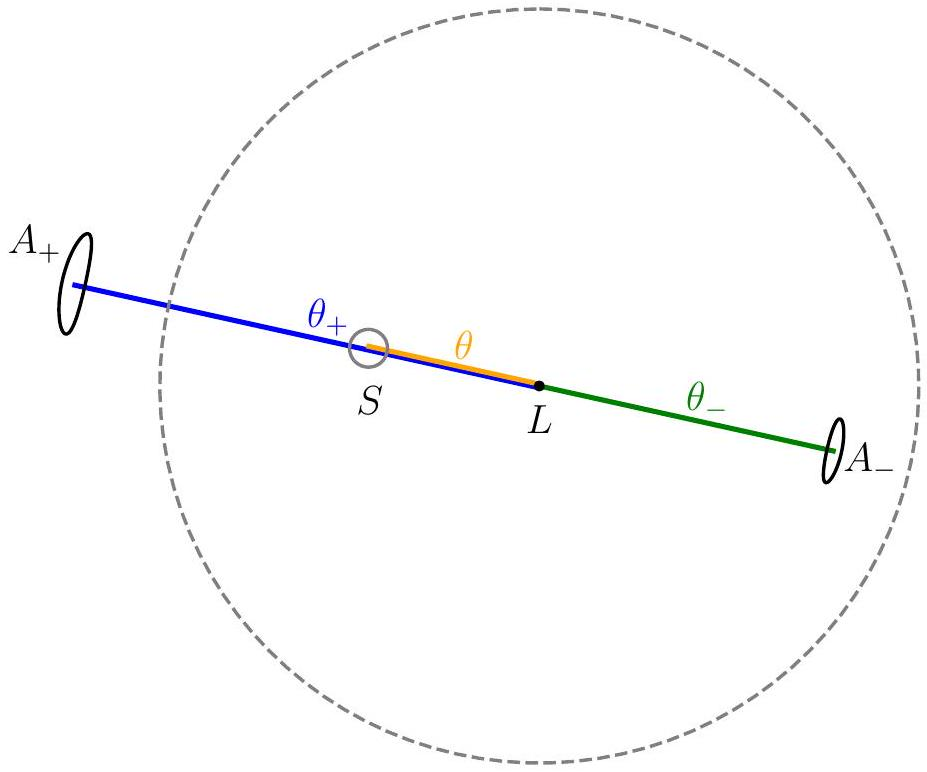
\includegraphics[max width=\textwidth, center]{2025_09_11_2a6858dd99d789184a35g-06}\\
(b) Current telescopes cannot normally resolve this pair of images, but only measure the position of the image centroid, i.e. the brightness-weighted mean of the positions of the two images. Derive an expression for the angular separation $\theta_{c}$ of the image centroid relative to the lens as a function of $u$ and $\theta_{\mathrm{E}}$.\\
(8 points)\\
(c) Derive an expression for the source deflection $\Delta \theta$, i.e. the difference between the location of the centroid and the unlensed position of the source, as a function of $u$ and $\theta_{\mathrm{E}}$. What is the source deflection when the lens and the source are nearly perfectly aligned ( $u \approx 0$ )?\\
(4 points)\\
The source and lens are moving relative to each other in the sky. Thus, both the total magnification of the images and the position of the centroid changes with time, resulting in observable photometric and astrometric microlensing effects. For now, we assume that the source-lens relative motion is rectilinear.

The plot below shows the light curve of the gravitational microlensing event OGLE-2011-BLG0462, discovered by the OGLE sky survey led by astronomers from the University of Warsaw. The solid line shows the best-fitting light curve model. The Einstein timescale of the event, i.e. the time needed for the source to move by one angular Einstein radius relative to the lens, was $t_{\mathrm{E}}=247$ days. The event peaked on 21 July 2011 (HJD $=2455763$ ). The minimal separation between the lens and the source was $u_{0} \approx 0$.\\
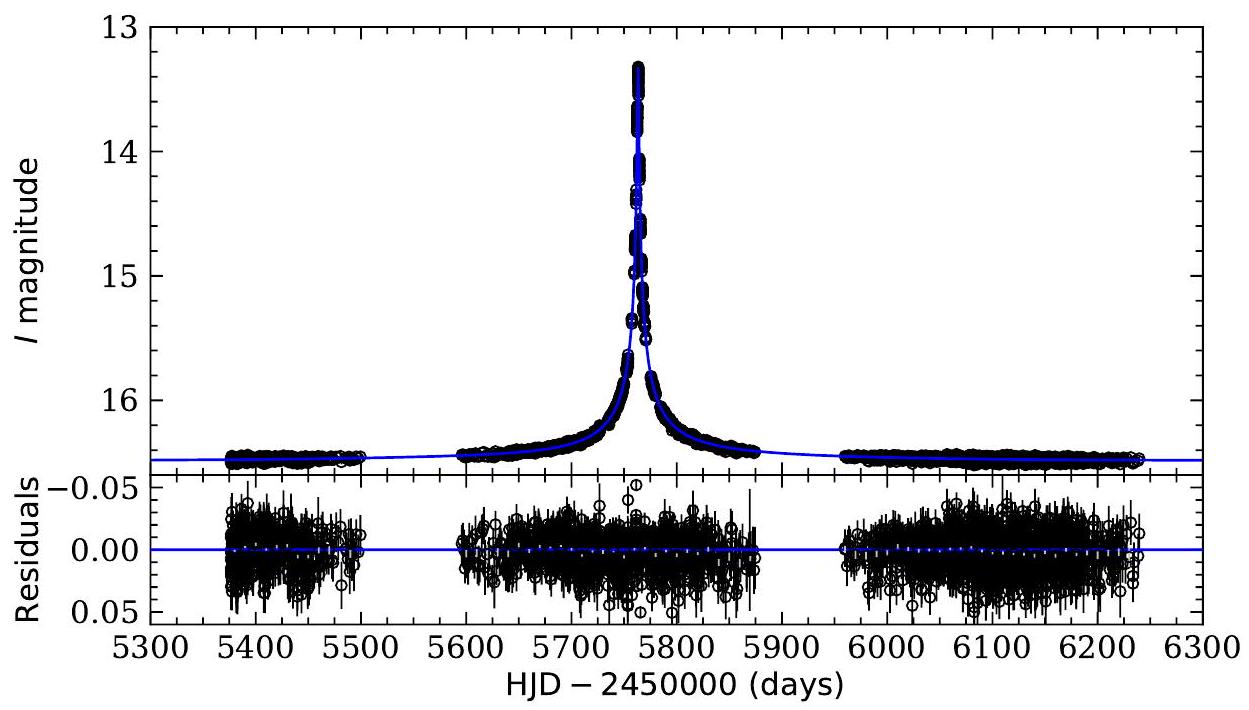
\includegraphics[max width=\textwidth, center]{2025_09_11_2a6858dd99d789184a35g-07}

The table below shows the measured positions of the source star against the background objects in the East and North directions based on images from the Hubble Space Telescope.

\begin{center}
\begin{tabular}{rrr}
\hline\hline
HJD & E position (mas) & N position (mas) \\
\hline
2455765.2 & $2.58 \pm 0.13$ & $7.29 \pm 0.16$ \\
2455865.7 & $2.32 \pm 0.12$ & $5.44 \pm 0.24$ \\
2456179.7 & $0.46 \pm 0.14$ & $1.62 \pm 0.08$ \\
2456195.8 & $0.88 \pm 0.36$ & $1.56 \pm 0.77$ \\
2456426.2 & $-1.02 \pm 0.21$ & $-0.94 \pm 0.12$ \\
2456587.7 & $-2.04 \pm 0.07$ & $-1.88 \pm 0.40$ \\
2456956.6 & $-4.54 \pm 0.25$ & $-5.16 \pm 0.29$ \\
2457995.2 & $-11.14 \pm 0.12$ & $-15.14 \pm 0.17$ \\
\hline
\end{tabular}
\end{center}

(d) Plot the measured positions of the source star against the background objects in the East and North directions as a function of time.\\
(10 points)\\
(e) The observed motion of the source star is the sum of two effects: rectilinear proper motion of the source and astrometric microlensing effects. Calculate the proper motion (in mas/year) of the source and its uncertainty in the East and North directions. (8 points)\\
(f) After subtracting the effects of proper motion from the data, calculate and plot the total resultant astrometric deflection as a function of $u$. Neglect the uncertainty of the proper motion determination.\\
(20 points)\\
(g) Analyse the data to determine the angular Einstein radius $\theta_{\mathrm{E}}$ of the event and its uncertainty. (Hint: it may be helpful to linearise the expression for $\Delta \theta$ ).\\
(16 points)\\
(h) For long-timescale events such as OGLE-2011-BLG-0462, the rectilinear approximation of the relative lens-source proper motion is not strictly true and the orbital motion of the Earth has to be taken into account. This allows measurement of a dimensionless quantity called the microlensing parallax, defined as $\pi_{\mathrm{E}}=\left(\pi_{l}-\pi_{s}\right) / \theta_{\mathrm{E}}$, where $\pi_{l}$ and $\pi_{s}$ are parallaxes of the lens and the source, respectively.

For this event $\pi_{\mathrm{E}}=0.095 \pm 0.009$. Rearrange the expression for $\theta_{\mathrm{E}}$ given earlier to calculate the mass of the lens in solar masses and its uncertainty.\\
(7 points)\\
(Total: 75 points)

\end{document}